\documentclass[12pt,a4paper]{article}
\usepackage[utf8]{inputenc}
\usepackage[ngerman]{babel}
\usepackage{graphicx}
\usepackage{booktabs} % Für Tabellen
\usepackage{caption}
\usepackage{amsmath}
\usepackage{enumitem} % Paket für bessere Nummerierung
\usepackage{csquotes} 


\usepackage{xcolor}
\usepackage{listings}
 
 
 \definecolor{codegreen}{rgb}{0,0.6,0}
 \definecolor{codegray}{rgb}{0.5,0.5,0.5}
 \definecolor{codepurple}{rgb}{0.58,0,0.82}
 \definecolor{backcolour}{rgb}{0.95,0.95,0.92}
 
 \lstdefinestyle{mystyle}{
 	backgroundcolor=\color{backcolour},
 	commentstyle=\color{codegreen},
 	keywordstyle=\color{magenta},
 	numberstyle=\tiny\color{codegray},
 	stringstyle=\color{codepurple},
 	basicstyle=\ttfamily\footnotesize,
 	breakatwhitespace=false,
 	breaklines=true,
 	captionpos=b,
 	keepspaces=true,
 	numbers=left,
 	numbersep=5pt,
 	showspaces=false,
 	showstringspaces=false,
 	showtabs=false,
 	tabsize=2
 }
 
 \lstset{style=mystyle}
 

\usepackage{tikz}
\usetikzlibrary{positioning}
\tikzstyle{block} = [rectangle, draw, fill=blue!20, text width=6em, text centered, rounded corners, minimum height=4em]
\tikzstyle{arrow} = [thick,-,>=stealth]


\usepackage{tikz}
\usepackage{hyperref} % Hinzugefügte Option

\usepackage[backend=biber, style=numeric]{biblatex}
\addbibresource{references.bib}
\begin{document}
	
		
		% Titelseite
		\begin{titlepage}
			\begin{center}
				\vspace*{1cm}
				\Huge
				Spracherkennung, Übersetzung und Textanalyse mit Google Cloud APIs
				
				
				\vspace{1.5cm}
				\LARGE
				M.Sc. Onur Yilmaz
				
				\vspace{1.5cm}
				\Large
				Angewandte Künstliche Intelligenz
				
				\vfill
				
				Schriftliche Ausarbeitung - Cloud Computing
				\vspace{0.5cm}
				\large
				Fachhochschule Südwestfalen
				\vspace{0.8cm}
				\Large
				\\
				Gutachter: Prof. Dr. Giefers
				\\
				\vspace{0.5cm}
				\large		
				\today
			\end{center}
		\end{titlepage}

\thispagestyle{empty}
\tableofcontents

\newpage
\section*{Einleitung}
In dieser Arbeit werden Technologien und Anwendungen aus dem Bereich der Sprach- und Textverarbeitung beleuchtet, die auf Google Cloud-Diensten aufbauen. Hierzu gehören die \textit{Cloud Speech API}, die \textit{Cloud Translation API}, die \textit{Natural Language API} und die \textit{Text-to-Speech API} \cite{googlecloudskills2023}.
\\ \\
Im ersten Abschnitt, der sich auf \cite{giefers2023cloud} bezieht, wird eine kurze Einführung in die Konzepte des Cloud Computings sowie der API-Integration im Zusammenhang mit NLP-Technologien gegeben, sowie die Interaktion mit der Google Cloud API erläutert.
\\ \\
Der Abschnitt \textit{Spracherkennung und -transkription} fokussiert sich auf die \textit{Cloud Speech API}, die die Transkription von Audio in Text ermöglicht, und die Methoden zur Messung und Verbesserung der Sprachgenauigkeit.
\\ \\
In der \textit{Sprachübersetzung} wird die \textit{Cloud Translation API} behandelt, die den Prozess der Übersetzung von Texten in verschiedene Sprachen ermöglicht.
\\ \\
Der Bereich \textit{Textanalyse} befasst sich mit der \textit{Natural Language API}, die Techniken zur Klassifizierung von Text in Kategorien und zur Analyse von Entitäten und Sentiments bietet.
\\ \\
Die Arbeit dient nicht nur als theoretischer Überblick, sondern bietet auch praktische Einblicke und Anleitungen zur Verwendung dieser Tools. Dabei werden unterschiedliche Schwierigkeitsgrade und Themenbereiche abgedeckt, um einen umfassenden Einblick in die Möglichkeiten der Sprach- und Textverarbeitung mit Google Cloud zu bieten.

	
\newpage

\section{Cloud Computing und NLP-Technologien}

\subsection{Cloud Computing im Kontext von NLP}
Cloud Computing bezeichnet die Bereitstellung von IT-Ressourcen wie Rechenleistung, Speicherplatz und Anwendungen über das Internet. Anstatt Ressourcen physisch vor Ort zu haben, ermöglicht Cloud Computing den Zugriff auf diese Ressourcen in großen Datenzentren. Dies bietet Unternehmen und Einzelpersonen Flexibilität, Skalierbarkeit und oft Kosteneffizienz. Im Kontext der natürlichen Sprachverarbeitung (NLP) revolutioniert Cloud Computing die Verarbeitung, Analyse und Interpretation großer Mengen von Sprachdaten. Es ermöglicht den Zugriff auf leistungsstarke und skalierbare Ressourcen, die NLP-Projekte effizient und effektiv durchführen.
\subsection{APIs und ihre Rolle im NLP}
Wenn man über Cloud spricht, ist eine der Hauptinteraktionen die Verwendung von APIs. 
\\ \\
Eine \textbf{\textit{API (Application Programming Interface)}} dient als Schnittstelle, die es Entwicklern ermöglicht, bestimmte Funktionen eines Programms oder einer Plattform zu nutzen, ohne sich mit den internen Details auseinandersetzen zu müssen. 
\\ \\
Das Aufrufen einer API, oft als \enquote{API-Anfrage} (\textit{im engl. request})  bezeichnet und ist der Prozess, bei dem ein Programm oder eine Anwendung eine Anforderung an einen Server sendet und eine Antwort zurückerhält.

\ \\ \\
\begin{tikzpicture}
	% Anwendung
	\node[draw,rectangle,fill=blue!20,minimum width=3cm,minimum height=2cm] (app) {Anwendung};
	% API-Server
	\node[draw,rectangle,fill=red!20,minimum width=3cm,minimum height=2cm, right=5cm of app] (api) {API-Server};
	
	% Pfeile für Anfrage und Antwort
	\draw[->, thick] (app.east) -- node[above]{Anfrage} (api.west);
	\draw[->, thick] (api.west) -- node[below]{Antwort} (app.east);
\end{tikzpicture}
\ \\ \\
Ein Großteil der modernen APIs, insbesondere im Cloud-Bereich, basiert auf dem Prinzip von REST (Representational State Transfer).\\ \\
\textit{\textbf{RESTful APIs}} nutzen Standard-HTTP-Methoden und bieten einen einheitlichen und vorhersehbaren Mechanismus, um mit dem Server zu interagieren. Dies erleichtert die Integration in Anwendungen und ermöglicht eine breitere Kompatibilität zwischen verschiedenen Systemen.
\\ \\
Im Kontext von NLP und Cloud Computing bieten RESTful APIs eine schnelle, zuverlässige und sichere Möglichkeit, auf leistungsstarke NLP-Modelle und -Dienste zuzugreifen. Sie ermöglichen es Entwicklern, Daten in Echtzeit zu verarbeiten und sofortige Analysen oder Antworten zu erhalten.
Zum Beispiel Textdaten zu senden und als Antwort eine Analyse oder Übersetzung dieses Textes zu erhalten, wäre eine beliebte und heutzutage häufig gebrauchte Anwendung ist. \\
\begin{center}
	\begin{tikzpicture}
		\node[draw, rectangle, fill=blue!20, minimum width=1cm, minimum height=1cm] (app) {NLP-Anwendung};
		\node[draw, rectangle, fill=red!20, minimum width=1.5cm, minimum height=1.5cm, right=of app, xshift=2cm] (api) {API};
		\node[draw, rectangle, fill=green!20, minimum width=1cm, minimum height=1cm, right=of api, xshift=2cm] (server) {NLP-Modell};
		
		\draw[->] (app) -- (api) node[midway, above] {Texteingabe};
		\draw[->] (api) -- (server) node[midway, above] {Verarbeitung};
		\draw[->] (server) -- (api) node[midway, below] {Antwort};
		\draw[->] (api) -- (app) node[midway, below] {Analyse};
	\end{tikzpicture}
\end{center}
\subsection{Interaktion mit der Google Cloud API}
Die Google Cloud Plattform bietet eine Vielzahl von RESTful APIs, die speziell für NLP-Aufgaben konzipiert sind. Diese APIs profitieren von der leistungsstarken Infrastruktur von Google, welche es Entwicklern ermöglicht, auf fortschrittliche NLP-Funktionen zuzugreifen. Für den Zugriff auf die Google Cloud APIs ist eine Authentifizierung erforderlich, die häufig über \textbf{\textit{API-Keys}} erfolgt. Sobald die Authentifizierung erfolgreich ist, können Entwickler Daten senden, diese verarbeiten lassen und die Ergebnisse für ihre spezifischen Anwendungen oder Analysen abrufen.


%%%%%%%%%%%%%%%%%%%%%%%%%%%%%%%%%%%%%%%%%%%%%%%%%%%%%%%%%%%%%%%%%%%%%%%%%%%%%%%%%%%%%%%%%%%%%%
\newpage

\section{Spracherkennung und Transkription}
In diesem Abschnitt behandeln wir den Prozess der Spracherkennung und Texttranskription (siehe \cite{towards}), einschließlich der Nutzung der Google Cloud Speech API zur Konvertierung von gesprochener Sprache in Textform \cite{speechtotext2023}. Um hochwertige Transkriptionen zu erhalten, werden wir außerdem auf die Messung und Verbesserung der Genauigkeit bei der Spracherkennung eingehen. Hierbei stützen wir uns auf \cite{speechaccuracy2023}.
\subsection{Sprache-zu-Text-Prozess}
Die Automatische Spracherkennung (ASR), auch als maschinelles Transkribieren oder Sprache-zu-Text bezeichnet, nutzt fortschrittliche Methoden des maschinellen Lernens, um gesprochene Audioinhalte in geschriebenen Text zu verwandeln. Die Einsatzmöglichkeiten sind äußerst vielfältig und reichen von der Erstellung von Untertiteln über die Unterstützung virtueller Assistenten bis hin zur Realisierung interaktiver Sprachsysteme.
\\ \\
Der Prozess beginnt mit der Erfassung der gesprochenen Sprache, sei es mittels eines Mikrofons oder anderer Audioeingaben. Die aufgenommenen Audiosignale werden in diskrete Zeitfenster von typischerweise 10 bis 25 ms unterteilt, die als Sprachrahmen bezeichnet werden. Diese Sprachrahmen fungieren als die elementaren Bausteine, auf denen das ASR-System operiert.
\\ \\
In der nächsten Phase erfolgt die akustische Modellierung. Dieser Schritt umfasst die Analyse der individuellen Sprachrahmen mit dem Ziel, die darin enthaltenen zugrundeliegenden Klänge, als \textit{Phoneme} bekannt, zu identifizieren. Phoneme sind die kleinsten distinkten sprachlichen Einheiten, die den Bausteinen der Wörter zugrunde liegen. Das akustische Modell nutzt ein Trainingskorpus, um auf akkurate Weise die Charakteristiken der Klangmuster in den Audiosignalen zu erfassen und diesen Mustern die entsprechenden Phoneme zuzuordnen.
\\ \\
In der Anschlussphase durchläuft die erkannte Phonemsequenz das Sprachmodell. Das Sprachmodell nutzt die geordnete Abfolge der Phoneme, um kohärente Wörter und Sätze zu generieren, die den erkannten Lauten entsprechen. Dieser Schritt stellt einen essentiellen Bestandteil dar, um die gesprochene Äußerung in einen verständlichen und grammatikalisch korrekten schriftlichen Ausdruck zu transformieren. Am Ende dieses Prozesses stellt das ASR-System den transkribierten Text als Endergebnis dar. 
\\ \\ 
Hier sieht man eine vereinfachte Darstellung dieses Modelles:
\begin{figure}[h!]
	\centering
	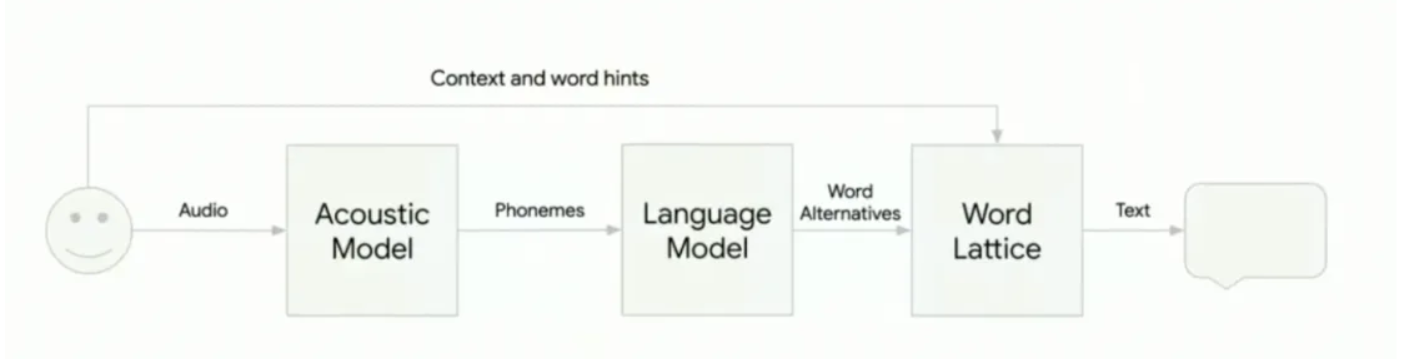
\includegraphics[width=1\linewidth]{../images/STT}
	\caption{\textit{Speech-to-Text} - Prozess}
	\label{fig:stt}
\end{figure}
\subsubsection{Messung und Verbesserung der Sprachgenauigkeit}
Die Genauigkeit der Spracherkennung kann auf verschiedene Arten gemessen werden. Je nach Bedarf können mehrere Metriken verwendet werden. Der branchenübliche Vergleich erfolgt jedoch oft mithilfe des Wortfehlerquotienten (Word Error Rate, WER). Die Wortfehlerquote misst den Prozentsatz falscher Transkriptionen im gesamten Satz. Eine niedrigere WER bedeutet daher, dass das System genauer ist.
\\ \\
In Bezug auf die Genauigkeit der ASR sehen Sie möglicherweise auch den Begriff \textit{Ground Truth}. Ground Truth bezieht sich auf die zu 100\% genaue (in der Regel menschliche) Transkription, mit der Sie die Genauigkeit vergleichen.
\\ \\
Die Wortfehlerquote setzt sich aus drei Arten von Transkriptionsfehlern zusammen, die auftreten können:

\begin{itemize}
	\item Einfügefehler (I): Wörter, die in der Transkription vorhanden sind, jedoch nicht in der Ground-Truth-Transkription.
	\item Substitutionsfehler (S): Wörter, die sowohl in der Transkription als auch in der Ground Truth vorhanden sind, aber nicht korrekt transkribiert wurden.
	\item Löschungsfehler (D): Wörter, die in der Transkription fehlen, jedoch in der Ground-Truth-Transkription vorhanden sind.
\end{itemize}
\ \\
Die Formel für die WER lautet: 
\[ \text{WER} = \frac{S + D + I}{N} \]
\\
Die Anzahl der Fehler jeder der drei Arten wird summiert und durch die Gesamtzahl der Wörter (N) in der Ground-Truth-Transkription geteilt, um die Wortfehlerquote (WER) zu ermitteln. Dies bedeutet, dass die WER in Situationen mit sehr geringer Genauigkeit größer als 100\% sein kann.
\subsection{Cloud Speech API}
\subsubsection{Erstellen eines API-Keys}
\label{subsubsec:generate-key} 
Wir beschreiben nun die Schritte, um einen API-Schlüssel zu erstellen und der uns über der SSH bereitgestellten Linux-Instanz verbinden zu können.
\\ \\
Um die Cloud Speech API mithilfe von \texttt{curl} anzusprechen, benötigen wir einen API-Schlüssel, der in der Anfrage-URL übergeben wird. Hier sind die Schritte zur Erstellung eines API-Schlüssels:
\begin{enumerate}
	\item Wir klicken im Navigationsmenü zu \enquote{APIs \& Services $>$ Anmeldedaten}.
	
	\item Klicken anschließend auf \enquote{Zugangsdaten erstellen (\textit{im engl. Credentials})} und wählen \enquote{API-KEY} aus.
	
	\item Bewahren die erstellte API-Schlüssel sicher auf, da wir diesen später in unserer Entwicklungsumgebung als Variable verwenden werden.
	
	\item Wir klicken anschließend auf \enquote{Schließen}.
\end{enumerate}
\begin{figure}[h!]
	\centering
	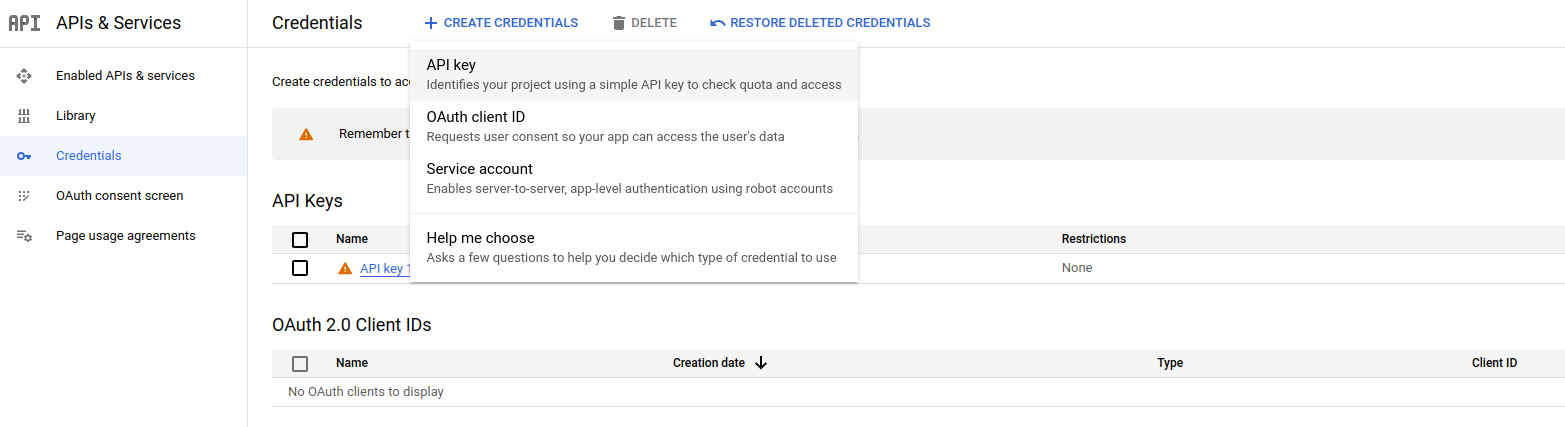
\includegraphics[width=1\linewidth]{../images/GCP_CREATE_API}
	\caption{Erstellen eines API-KEYs in GCP}
	\label{fig:gcpcreateapi}
\end{figure}
\ \\
Um die nächsten Schritte auszuführen, verbinden wir uns mit der Ihnen bereitgestellten Linux-Instanz über SSH:
\begin{enumerate}
	\item Navigieren im Navigationsmenü zu \enquote{Compute Engine $>$ VM-Instanzen}.
	
	\item Suchen die Linux-Instanz VM in der Liste der VM-Instanzen. 
	
	\item Klicken rechts neben dem Namen der Linux-Instanz auf \enquote{SSH}, um eine interaktive Shell zu öffnen. Diese Shell verwenden wir, um die nächsten Schritte auszuführen.

\begin{figure}[h!]
	\centering
	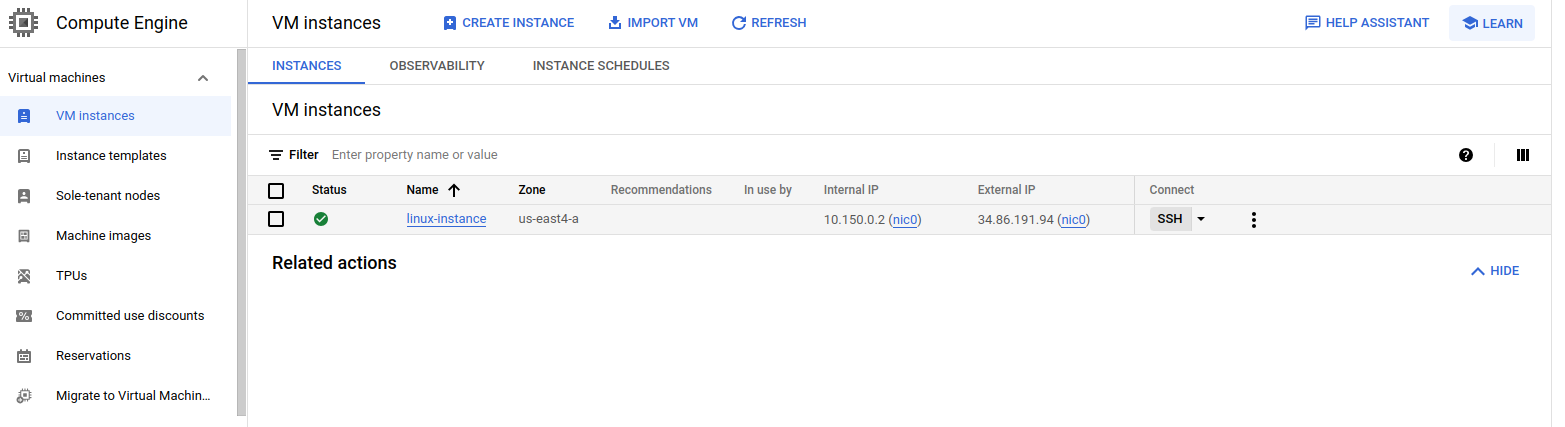
\includegraphics[width=1\linewidth]{../images/VM_Instances}
	\caption{VM Instanz}
	\label{fig:vminstances}
\end{figure}

	\item In der geöffneten SSH-Shell führen wir den folgenden Befehl aus und ersetzen den KEY durch den von uns zuvor erstellten API-Schlüssel:

\begin{figure}[h!]
	\centering
	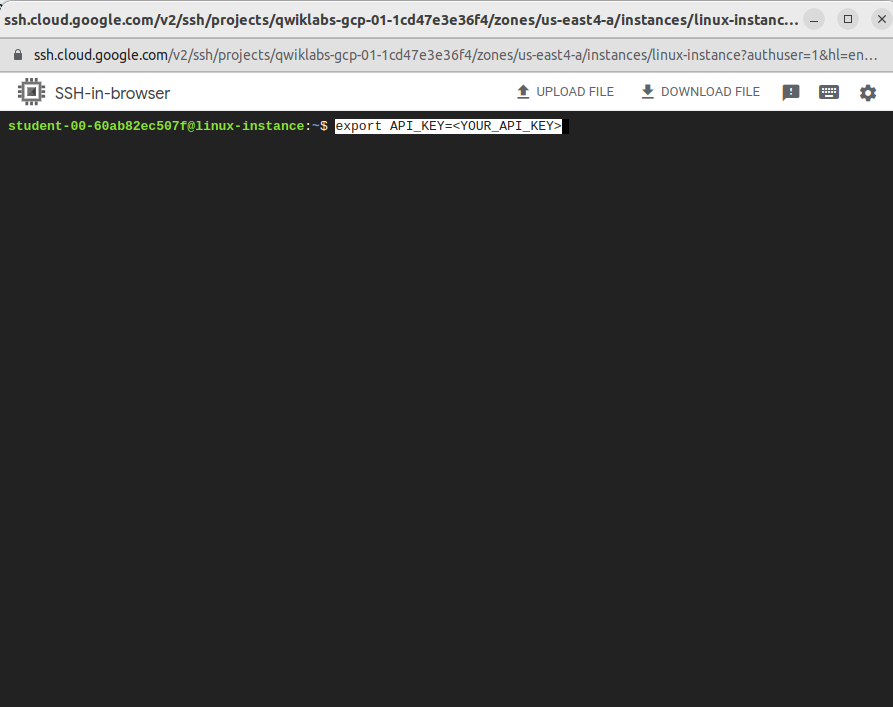
\includegraphics[width=0.7\linewidth]{../images/SSH}
	\label{fig:ssh}
\end{figure}
\end{enumerate}
\ \\ \\
Der nächste Schritt ist die Verwendung von \texttt{curl}, um eine Anfrage an die Cloud Speech API zu senden und die gewünschten Transkriptionen zu erhalten. 
\subsubsection{Erstellen der API-Anfrage}
\begin{enumerate}
\item Wir erstellen unsere Anfrage an die API in einer \texttt{request.json}-Datei. Die Datei \texttt{request.json} kann wie folgt erstellt werden:
\begin{center}
\verb|touch request.json|
\end{center}
\item Anschließend öffnen wir die Datei mit unserem bevorzugten Editor (nano, vim, emacs) und fügen Folgendes zu unserer \texttt{request.json}-Datei hinzu:
\begin{figure}[h!]
\centering
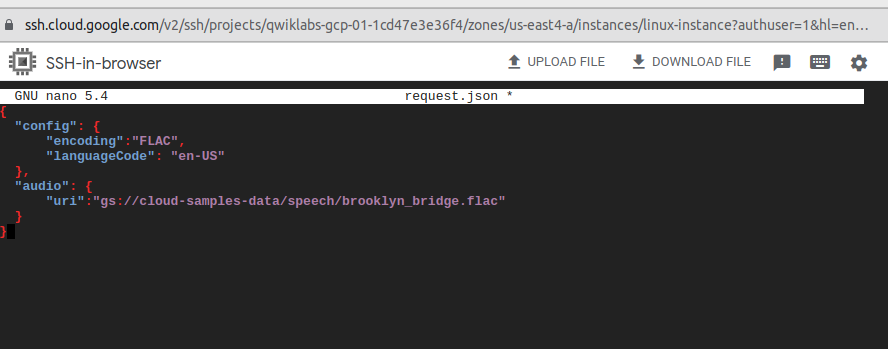
\includegraphics[width=0.9\linewidth]{../images/request_json}
\label{fig:requestjson}
\end{figure}
\ \\
Hier obiger Code noch einmal übersichtlich dargestellt:
\begin{verbatim}
	{
		"config": {
			"encoding":"FLAC",
			"languageCode": "en-US"
		},
	
		"audio": {
			"uri":"gs://cloud-samples-data/speech/brooklyn_bridge.flac"
		}
	}
\end{verbatim}
Nachdem wir uns den obigen JSON-Code erstellt haben, werfen wir einen Blick über die einzelnen Bestandteile
\begin{itemize}
	\item \enquote{config}: Dies ist ein Objekt, das Konfigurationseinstellungen enthält.
	
	\item \enquote{encoding}: \enquote{FLAC}: Dies legt das Encoding (Datenformat) für den Audiodatenstrom fest. In diesem Fall wird das FLAC-Format verwendet, das ein verlustfreies Audioformat ist.
	
	\item \enquote{languageCode}: \enquote{en-US}: Dies gibt den Sprachcode an. Hier ist es \enquote{en-US}, was auf US-Englisch hinweist.
	
	\item \enquote{audio}: Dies ist ebenfalls ein Objekt, das Informationen über die Audiodaten enthält.
	
	\item \enquote{uri}: \enquote{gs://cloud-samples-data/speech/brooklyn\_bridge.flac}: Dies ist die URI (Uniform Resource Identifier) oder der Pfad zum Audiofile. In diesem Fall handelt es sich um eine Audioaufnahme der Brooklyn Bridge im FLAC-Format, die in der Google Cloud Storage (gs) gespeichert ist.
\end{itemize}
\end{enumerate}


\subsubsection{Aufrufen der API}
Um die API aufzurufen, müssen Sie den Anfragekörper zusammen mit der API-Schlüssel-Umgebungsvariable an die API übergeben. Dies kann mit dem folgenden \texttt{curl}-Befehl erledigt werden (alles in einer einzelnen Befehlszeile):

\begin{figure}[h!]
	\centering
	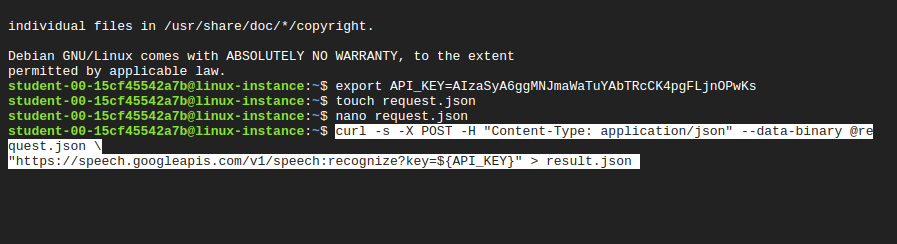
\includegraphics[width=1\linewidth]{../images/curl}
\end{figure}
\ \\
Hier noch einmal übersichtlich dargestellt:
\begin{verbatim}
curl -s -X POST -H "Content-Type: application/json" 
--data-binary @request.json \
"https://speech.googleapis.com/v1/speech:recognize?key=${API_KEY}" 
> result.json
\end{verbatim}
\ \\
Es handelt sich um einen \texttt{curl}-Befehl, der eine POST-Anfrage an die Google Cloud Speech-to-Text API sendet. Die Optionen \texttt{-s} und \texttt{-X POST} setzen den Befehl auf den silent-Modus und legen die Anfragemethode auf POST fest. Der Header \texttt{"Content-Type: application/json"} gibt den Medientyp der Anfrage an. Die Option \texttt{--data-binary @request.json} überträgt den Inhalt der Datei \texttt{request.json} als Anfragekörper. Die URL enthält den Endpunkt der API, und der Platzhalter \texttt{\${API\_KEY}} wird durch den tatsächlichen API-Schlüssel ersetzt. Anschließend wird die Antwort der API in einer Datei namens \texttt{result.json} gespeichert.
\\ \\
Mit dem Befehl \verb|cat result.json| erhält man die folgende Ausgabe: 
\begin{figure}[h!]
	\centering
	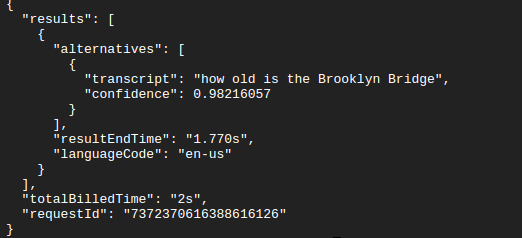
\includegraphics[width=1\linewidth]{../images/ergebnisse}
	\label{fig:ergebnisse}
\end{figure}
\ \\
Der Wert des \enquote{transcript} gibt die Texttranskription der Audio-Datei durch die Sprach-API wieder, während der \enquote{confidence}-Wert angibt, wie sicher die API ist, dass die Audio-Datei korrekt transkribiert wurde. 
\\ \\ 
Um die Google Speech-to-Text API in unserer eigenen Entwicklungsumgebung zu verwenden, ist es notwendig, zuerst das erforderliche Paket über pip herunterzuladen. Anschließend können wir den folgenden Python-Code verwenden, um die API zu nutzen. Dabei übergeben wir die Credentials aus der JSON-Datei und rufen die recognize-Funktion auf, um die Spracherkennung durchzuführen:
Die Funktion wird auf die selbe FLAC-Audiodatei\footnote{Auf   \url{https://github.com/ONURYI/Sprache-Text-und-Uebersetzung-mit-GCP-APIs} herunter ladbar} angewandt.
\
\begin{lstlisting}[language=Python,numbers = none]
	from google.cloud import speech
	
	client = speech.SpeechClient.from_service_account_json('YOUR.json')
	
	config = speech.RecognitionConfig(
	encoding=speech.RecognitionConfig.AudioEncoding.FLAC,
	language_code='en-US',   
	)
	
	with open('speech_brooklyn_bridge.flac', 'rb') as audio_file:
	content = audio_file.read()
	
	audio = speech.RecognitionAudio(content=content)
	response = client.recognize(config=config, audio=audio)
	
	for result in response.results:
	transcript = result.alternatives[0].transcript
	confidence = result.alternatives[0].confidence
	
	print('transcript: {}'.format(transcript))
	print('confidence: {}'.format(confidence))
\end{lstlisting}
Ausgabe: 
\begin{center}
	\verb|>> Transkript: how old is the Brooklyn Bridge| 
	\verb|confidence: 0.9821605682373047|
\textit{}\end{center}
\  \\ 
Zum Vergleich, schauen wir uns nun einmal das von OpenAI bereitgestellte ASR Modell, namens \textbf{\textit{Whisper AI}}(zugehörige Paper siehe \cite{radford2022robust}) an, welche mithilfe des Paketverwalters pip von Python installiert werden:

\begin{verbatim}
!pip install git+https://github.com/openai/whisper.git 
\end{verbatim}

\begin{lstlisting}[language=Python,numbers = none]
import whisper 

model = whisper.load_model('base')
model.transcribe('speech_brooklyn_bridge.flac',fp16=False)
\end{lstlisting}
\ \\
Und erhalten die folgende Ausgabe
\begin{verbatim}
	{'text': ' How old is the Brooklyn Bridge?',
		'segments': [{'id': 0,
			'seek': 0,
			'start': 0.0,
			'end': 1.76,
			'text': ' How old is the Brooklyn Bridge?',
			'tokens': [50364, 1012, 1331, 307, 264, 21872, 18917, 30, 50452],
			'temperature': 0.0,
			'avg_logprob': -0.3769610643386841,
			'compression_ratio': 0.8378378378378378,
			'no_speech_prob': 0.019619377329945564}],
		'language': 'en'}
\end{verbatim}
\ \\
Hier erkennen wir ebenfalls, dass die Sprache präzise transkribiert wird und auch die korrekte Groß- und Kleinschreibung berücksichtigt wird. Allerdings fehlt uns eine Einschätzung der \textit{Confidence} seitens des Modells.

%%%%%%%%%%%%%%%%%%%%%%%%%%%%%%%%%%%%%%%%%%%%%%%%%%%%%%%%%%%%%%%%%%%%%%%%%%%%%%%%%%%%%%%%%%%%%%

\newpage
\section{Sprachübersetzung}

In diesem Abschnitt wird nun die Erkennung und Übersetzung von Texten behandelt (siehe  \cite{tunstall2022natural}). Hierbei wird ebenfalls auf die Möglichkeiten der \textit{Cloud Translation API} von Google Cloud eingegangen (siehe \cite{cloudtranslation2023}).
\subsection{Übersetzung von Texten}
Die Übersetzung von Texten ist eine fundamentale Anwendung im NLP, bei der das Ziel darin besteht, Texte von einer Quellsprache in eine Zielsprache zu übertragen. Ein Schlüsselkonzept, das hierbei eine wichtige Rolle spielt, ist das \textbf{Sequence-to-Sequence-Modell}.
\\ \\
Letzteres ist eine weitverbreitete Architektur in der NLP, die speziell für die Übersetzung von Texten entwickelt wurde. 
\\ \\
Es besteht aus zwei grundlegenden Teilen:
\\ \\
\textbf{Encoder:} Der Encoder nimmt den Eingabetext in der Quellsprache auf, analysiert ihn und erstellt eine kompakte Repräsentation des Textes. Diese Repräsentation, oft als "Kontextvektor" bezeichnet, erfasst die semantischen und syntaktischen Eigenschaften des Eingabetextes.
\\ \\
\textbf{Decoder:} Der Decoder verwendet den Kontextvektor des Encoders, um schrittweise den Text in der Zielsprache zu generieren. Während des Generierungsprozesses greift der Decoder auf den Kontextvektor und die bereits erzeugten Teile des Ausgabetextes zurück, um den nächsten Schritt der Übersetzung zu bestimmen.
\ \\
\begin{center}
	\begin{tikzpicture}[node distance=2cm]
		% Nodes
		\node [rectangle, draw, minimum width=3cm] (encoder) {Encoder};
		\node [rectangle, below of=encoder] (context) {Kontextvektor};
		\node [rectangle, draw, minimum width=3cm, below of=context] (decoder) {Decoder};
		
		% Arrows
		\draw [-latex] (encoder) -- (context);
		\draw [-latex] (context) -- (decoder);
	\end{tikzpicture}
\end{center}
Wir versuchen das Sequence-to-Sequence-Modell noch einmal mit einem Beispiel zu verdeutlichen.
\ \\ 
Angenommen, wir haben die englischen und deutschen Sätze;
\\ \\
Englisch: \enquote{How old is the Brooklyn Bridge?}
\\  \\
Deutsch: \enquote{Wie alt ist die Brooklyn Bridge?}
\\ \\
Und unser Ziel ist es, vom englischen ins deutsche zu übersetzen. Folgende Schritte werden hier nun durchlaufen: \\
\begin{enumerate}
	\item \textbf{Tokenisierung:} \\
	Wir teilen die Sätze in Wörter oder Satzzeichen auf:
	\begin{itemize}
		\item Englisch: [\enquote{How}, \enquote{old}, \enquote{is}, \enquote{the}, \enquote{Brooklyn}, \enquote{Bridge}, \enquote{?}]
		\item Deutsch: [\enquote{Wie}, \enquote{alt}, \enquote{ist}, \enquote{die}, \enquote{Brooklyn}, \enquote{Bridge}, \enquote{?}]
	\end{itemize}
	
	\item \textbf{Vokabular erstellen:} \\
	Wir erstellen Vokabulare für Englisch und Deutsch:
	\begin{itemize}
		\item Englisches Vokabular: [\enquote{How}, \enquote{old}, \enquote{is}, \enquote{the}, \enquote{Brooklyn}, \enquote{Bridge}, \enquote{?}, ...]
		\item Deutsches Vokabular: [\enquote{Wie}, \enquote{alt}, \enquote{ist}, \enquote{die}, \enquote{Brooklyn}, \enquote{Bridge}, \enquote{?}, ...]
	\end{itemize}
	
	\item \textbf{Token-IDs zuweisen:} \\
	Jedes Wort wird einer numerischen ID\footnote{Exemplarisch willkürliche Darstellung.} zugeordnet:
	\begin{itemize}
		\item Englische Token-IDs: [101, 102, 103, 104, 105, 106, 107]
		\item Deutsche Token-IDs: [201, 202, 203, 204, 205, 206, 207]
	\end{itemize}
	
	\item \textbf{Training:} \\
	Das Modell wird mit den englischen Token-IDs als Eingabe und den deutschen Token-IDs als Ziel trainiert. Der Encoder verarbeitet den englischen Satz und erzeugt einen Kontextvektor. 
	
	\item \textbf{Übersetzung:} \\
	Der Decoder nutzt diesen Kontextvektor, um den deutschen Satz zu generieren.
\end{enumerate}
\ \\
Dies ist nur ein sehr stark vereinfachte Darstellung. In der Praxis werden häufig auf fortschrittliche neuronale Netzwerkarchitekturen wie RNNs, LSTMs und \textit{Attention Layers} zurückgegriffen. Letzteres zeichnet sich durch die Fähigkeit aus, den Kontext eines Satzes zu erfassen.
\subsection{Cloud Translation API}
Die Schritte zur Erstellung eines API-KEYs sind identisch mit dem in \ref{subsubsec:generate-key} Ablauf beschrieben Prozess.
\\ \\
Wir wollen hier nun den folgenden Text - \enquote{My name is Steve} ins Spanische übersetzen, hierzu übergeben wirden zu übersetzenden Text zusammen mit der API-Schlüssel-Umgebungsvariable an die Übersetzungs-API mithilfe des folgenden Curl-Befehls, direkt in die Cloud Shell ein.
\begin{center}
	\begin{verbatim}
		TEXT="My%20name%20is%20Steve"
		curl "https://translation.googleapis.com/language/translate/
		v2?target=es&key=${API_KEY}&q=${TEXT}"
	\end{verbatim}
\end{center}
\begin{figure}[h!]
	\centering
	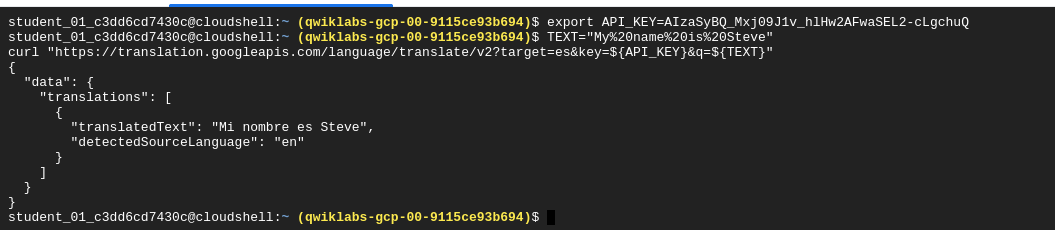
\includegraphics[width=1\linewidth]{../images/translation_API}
	\label{fig:translationapi}
\end{figure}
\url{"My%20name%20is%20Steve"} ist URL-codiert. Die URL-Codierung ist eine Methode, um Sonderzeichen und Leerzeichen in einer URL darzustellen. \\Unser Ergebnis lautet dann wie folgt:
\begin{figure}[h!]
	\centering
	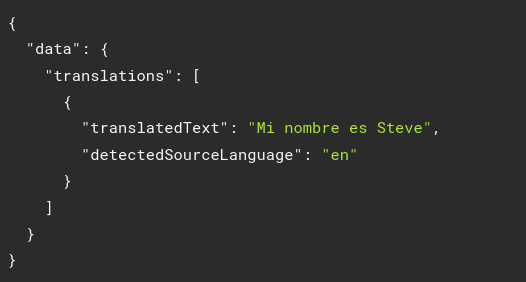
\includegraphics[width=0.7\linewidth]{../images/result_translate}
	\label{fig:resulttranslate}
\end{figure}
\ \\
Zusätzlich zur Übersetzung von Texten kann die Übersetzungs-API auch die Sprache des Textes erkennen. Hierzu geben wir 
\begin{verbatim}
	NEW_TEXT="Meu%20nome%20é%20Steven"
	curl "https://translation.googleapis.com/language/translate/
	v2/detect?key=${API_KEY}&q=${NEW_TEXT}"
\end{verbatim}
ein und erhalten die folgende Ausgabe:
\begin{figure}[h!]
	\centering
	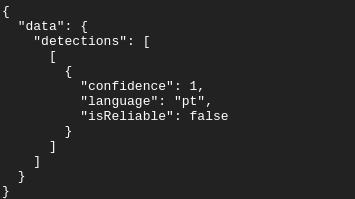
\includegraphics[width=0.7\linewidth]{../images/result_port}
	\label{fig:resultport}
\end{figure}


%%%%%%%%%%%%%%%%%%%%%%%%%%%%%%%%%%%%%%%%%%%%%%%%%%%%%%%%%%%%%%%%%%%%%%%%%%%%%%%%%%%%%%%%%%%%%%



\newpage
\section{Textanalyse}
Im letzten Abschnitt liegt der Fokus auf die Textklassifizierung und insbesondere der Entitäts- und Sentimentsanalyse. Hierbei stützen wir uns auf \cite{tunstall2022natural}. Wir erörtern außerdem die Anwendungsmöglichkeiten der Natural Language API von Google Cloud, um eine umfassende Analyse von Texten durchzuführen und sie entsprechenden Kategorien zuzuordnen \cite{classtext2023}, sowie die allgemeine Stimmung zu identifizieren \cite{entitysentiment2023}.
\subsection{Klassifizierung von Text in Kategorien}
Die Textklassifizierung ermöglicht das Verständnis und die Verarbeitung menschlicher Sprache. Hierbei werden unstrukturierte Textdaten systematisch organisiert und in sinnvolle Kategorien eingeordnet. Dieser Prozess beruht auf der Analyse sprachlicher Merkmale, Schlüsselwörter, Grammatik und semantischer Zusammenhänge im Text.
\\ \\
Ein prägnantes Beispiel für NLP-Klassifizierung ist die automatische Sortierung von E-Mails in Ordner wie \enquote{Eingang}, \enquote{Werbung} oder \enquote{Wichtig}. Durch die Identifikation von Mustern und Charakteristika im Text erfolgt eine gezielte Zuordnung der E-Mails zu den entsprechenden Kategorien.
\subsection{Entitäten- und Sentimentanalyse}
Die Entitäten- und Sentimentanalyse erweitert die Textanalyse. Entitäten sind spezifische Objekte, wie Personen, Orte oder Organisationen, die im Text erwähnt werden. Die Entitätenanalyse identifiziert und klassifiziert solche Elemente, um eine tiefere strukturierte Darstellung des Textinhalts zu ermöglichen.
\\ \\
Gleichzeitig erfasst die Sentimentanalyse die emotionale Tonalität eines Textes, sei es positiv, neutral oder negativ. Sie basiert auf der Auswertung von Wörtern und Ausdrücken im Text und ermöglicht somit die Einschätzung der übergeordneten Stimmung oder Meinung.
\subsection{Natural Language API}
Die Schritte zur Erstellung des API-Schlüssels sind erneut identisch mit dem in \ref{subsubsec:generate-key} beschriebenem. Um sicherzustellen, dass diese auch tatsächlich aktiviert sind, können wir in der Suchleiste \textit{\enquote{language}} eingeben und sehen das die Aktivierung funktioniert hat.

\begin{figure}[h!]
	\centering
	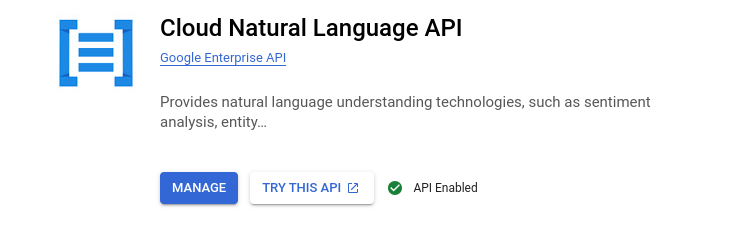
\includegraphics[width=0.8\linewidth]{../images/cloud_NLP_API}
	\label{fig:cloudnlpapi}
\end{figure}
\ \\
Mit Hilfe der \textbf{classifyText-Methode} der Natural Language API können wir Textdaten mithilfe eines einzigen API-Aufrufs in verschiedene Kategorien einteilen. Diese Methode liefert uns eine Liste von Inhaltskategorien, die auf ein Textdokument zutreffen.
\\ \\
Hierzu naviegeren wir wie in \ref{subsubsec:generate-key} zur Linux Instanz und erstellen folgende Anfrage:
\begin{verbatim}
	{
		"document":{
			"type":"PLAIN_TEXT",
			"content":"A Smoky Lobster Salad With a Tapa Twist. 
			This spin on the Spanish pulpo a la gallega skips the octopus, 
			but keeps the sea salt, olive oil, pimentón and boiled potatoes."
		}
	}
\end{verbatim}
Jetzt könnt ihr diesen Text mithilfe des folgenden curl-Befehls an die classifyText-Methode der Natural Language API senden
\begin{verbatim}
	curl "https://language.googleapis.com/v1/documents:
	classifyText?key=${API_KEY}" \ -s -X POST -H "Content-Type: 
	application/json" --data-binary @request.json > result.json
\end{verbatim}
und sehen, dass zwei Kategorien für diesen Text zurückgegeben worden sind:

\begin{itemize}
	\item /Food \& Drink/Cooking \& Recipes
	\item /Food \& Drink/Food/Meat \& Seafood
\end{itemize}
\newpage
\begin{figure}[h!]
	\centering
	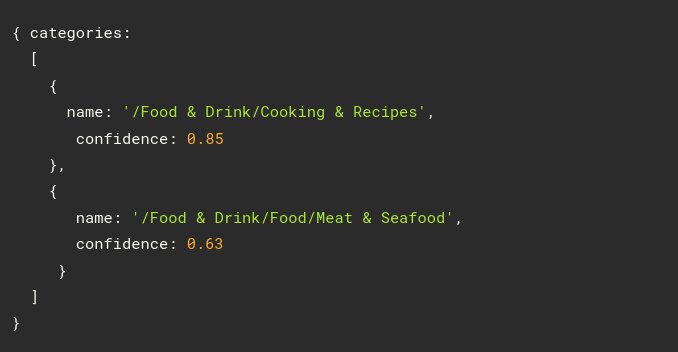
\includegraphics[width=0.8\linewidth]{../images/response_category}
	\label{fig:responsecategory}
\end{figure}
\ \\
Abschließend schauen wir nun die Entitäts - und Sentimentanalyse mit der Natural Language API an.




%%%%%%%%%%%%%%%%%%%%%%%%%%%%%%%%%%%%%%%%%%%%%%%%%%%%%%%%%%%%%%%%%%%%%%%%%%%%%%%%%%%%%%%%%%%%%%
\newpage
\
\newpage
\thispagestyle{empty}
\printbibliography

\end{document}
